%! Author = lazza
%! Date = 03/05/2022

\section{Instruction level parallelism}\label{sec:instruction-level-parallelism}
ILP: potential overlap of execution among unrelated instructions, possible if:
\begin{itemize}
    \item no structural hazards
    \item no raw, waw, war stalls
    \item no control hazards
\end{itemize}

\begin{center}
    Pipeline CPI = Ideal pipeline CPI + Structural Stalls +\\Data Hazards Stalls + Control Stalls
\end{center}

In the MIPS architecture the only possible structural hazards, WB-ID, where a register in the RF can be both written
and read, is solved by splitting the clock cycle in rising edge (WB) and falling edge (ID).


\begin{table}[h]
    \centering
    \begin{tabular}{|p{3cm}|p{3.5cm}|}
        \toprule
        \textbf{ILP} & \textbf{PP} \\
        \midrule
        overlap individual machine operations & separate processor getting separate chuncks of the program \\
        \midrule
        transparent to the user & nontransparent to the user \\
        \midrule
        goal: speed up & goal: speed up and quality up \\
        \bottomrule
    \end{tabular}
    \caption{ILP vs Parallel Processing}
    \label{tab:ILP-vs-PP}
\end{table}


\subsection{Complex Pipeline}\label{subsec:complex-pipeline}
WAR and WAW were not possible with ADD operation with integers, but MULT and DIV operations use floating point numbers.
A new stage introduced, the ISSUE stage, that allows for high performance in presence of:
\begin{itemize}
    \item long latency or partially pipeline floating-point units
    \item multiple function and memory units
    \item memory systems with variable access time
    \item precise exception
\end{itemize}

\begin{figure}[h]
    \centering
    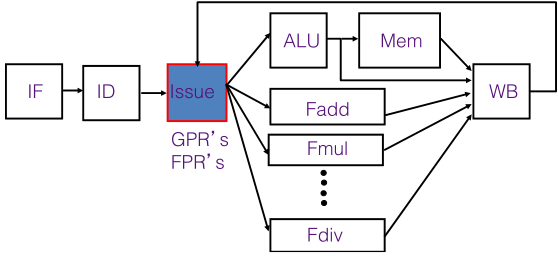
\includegraphics[scale = 0.4]{images/complex-pipeline}
    \caption{Complex pipeline}
    \label{fig:complex-pipeline}
\end{figure}

New hazards arise from variable latencies of different FUs:
\begin{itemize}
    \item Structural
    \begin{itemize}
        \item EX stage if some FPU or memory unit is not pipelined and takes more than one cycle.
        \item WB stage due to variable latencies of different functional units
    \end{itemize}
    \item Data
    \begin{itemize}
        \item WAW due to variable latencies of the FUs
    \end{itemize}
\end{itemize}

A solution would be delay the WB in order to have the same latency for all instructions but that would slow down too
much single cycle integer operations without forwarding.

\paragraph{When it is safe to issue an Instruction?} Things to consider before dispatching an instruction:
\begin{itemize}
    \item the required FU is available
    \item the input data is available
    \item it is safe to write the destination
    \item there is not a structural conflict at the WB stage
\end{itemize}

\paragraph{Assumptions} Of a general complex pipeline architecture:
\begin{itemize}
    \item all functional units are pipelined
    \item registers are read in ISSUE stage: we consider that a register is written (WB) in the first half of the clock
    cycle and read (IS) in the second half of the clock cycle
    \item no forwarding
    \item ALU operations take 1 clock cycle
    \item FP ALU operations take 2 clock cycles
    \item memory operations take 2 clock cycles
    \item write back unit has a single port
    \item instructions are fetched, decoded and issued in order
    \item an instruction will only enter the ISSUE stage if it does not cause a WAR or WAW hazard
    \item only one instruction can be issued at a time, and in the case multiple instructions are ready, the oldest
    one will go first
\end{itemize}


To reach higher performance more parallelism must be achieved, this cannot be done augmenting the CPI of the ideal
pipeline because it could create further problems with hazards.

Dependences must be detected and solved, and
instructions must be ordered (scheduled) so as to
achieve highest parallelism of execution compatible
with available resources.

Three types of dependencies:
\begin{itemize}
    \item data dependencies, RAW
    \item control dependencies
    \item name dependencies, two types:
    \begin{itemize}
        \item antidependencies, WAR
        \item output dependencies, WAW
    \end{itemize}
    Generated by the lack of registers.
\end{itemize}

Dependencies are a property of the program, while
hazards are a property of the pipeline.


The main techniques to eliminate dependencies are:
\begin{itemize}
    \item register renaming
    \item scheduling
    \begin{itemize}
        \item static, compiler
        \item dynamic, hardware
    \end{itemize}
\end{itemize}
%-> superscalar

Steps to exploit more ILP in terms of hardware optimization:
\begin{itemize}
    \item[\textrightarrow] sequential
    \begin{itemize}
        \item[$\hookrightarrow$] pipeline\\ single-issue in-order-execution
        \begin{itemize}
            \item[$\hookrightarrow$] dynamic scheduling\\ single-issue out-of-order execution
            \begin{itemize}
                \item[$\hookrightarrow$] superscalar\\ multiple-issue out-of-order execution
            \end{itemize}
        \end{itemize}
    \end{itemize}
\end{itemize}

\begin{figure}
    \centering
    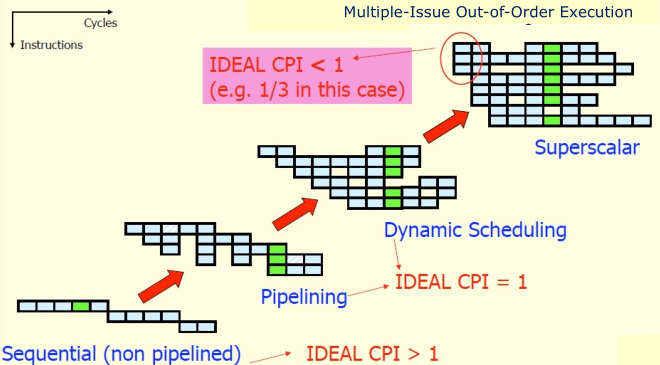
\includegraphics[scale = 0.4]{images/ILP-scheme}
    \caption{Instruction Level Parallelism}
    \label{fig:ILP-scheme}
\end{figure}
